\documentclass[10pt, a4paper]{article}

\usepackage[utf8]{inputenc}
\usepackage[english]{babel}
\usepackage{amsmath}
\usepackage{amsfonts}
\usepackage{csquotes}
\usepackage{bm}
\usepackage{indentfirst}
\usepackage{graphicx}
\usepackage{geometry}
\usepackage{minted}
\usepackage{hyperref}
\usepackage{subcaption}
\usepackage[font=small,labelfont=bf]{caption}

% \renewcommand{\familydefault}{\sfdefault} % <- much easier to proof-read in sans-serif, feel free to switch back to serifs before submitting :)

\usepackage[T1]{fontenc}
\usepackage{fourier}

\usepackage{algorithm}
\usepackage{algpseudocode}

\graphicspath{ {./images/} }
\geometry{a4paper,
    left=3cm,
    top=3cm,
    bottom=3cm,
    right=2.5cm
}


\title{{\Large \textbf{FYS-STK4155} Project 1} \\ 
            Regression analysis and resampling methods}
\author{João Inácio, Johan Andreas Fløisand, Jonathan Kings}
\date{\today}


\begin{document}

\maketitle

\section*{Introduction}

    Norway is known for its high mountains and deep valleys. With such a varied terrain, it would be interesting to see how well it could be approximated by a polynomial. In this project we aim to analyse exactly how well\footnote{In this project, we will let the mean squared error of the data and our model be a measurement of how well our model fits the data.} terrain data can be approximated by polynomials. To determine this, we will use three different regression methods: Ordinary Least Squares, Ridge and Lasso. We begin by analysing easier data, namely the \textit{Franke function}. The Franke function, $f:\mathbb{R}^2\to\mathbb{R}$, is given by
    \begin{align*}
    f(x,y) &= \frac{3}{4}\exp{\left(-\frac{(9x-2)^2}{4} - \frac{(9y-2)^2}{4}\right)}+\frac{3}{4}\exp{\left(-\frac{(9x+1)^2}{49}- \frac{(9y+1)}{10}\right)} \\
    &+\frac{1}{2}\exp{\left(-\frac{(9x-7)^2}{4} - \frac{(9y-3)^2}{4}\right)} -\frac{1}{5}\exp{\left(-(9x-4)^2 - (9y-7)^2\right) }.
    \end{align*}
    We will restrict ourselves to the region $[0,1]\times[0,1]$. We will also explore how a normally distributed (stochastic) noise affects our model. Our data will therefore be given by
    \begin{equation} \label{eq:data_model}
        \bm{z} = f(\bm{x},\bm{y}) + \bm{\epsilon},
    \end{equation}
    where \(\epsilon \sim N(0,\sigma^2)\) is the noise. For the entirety of our analysis of the Franke function, we use \(\sigma=0.25\).
    
    Assume now that we are given a data set \(\bm{z}=\begin{pmatrix}z_0 & z_1 & \ldots & z_{n-1}\end{pmatrix}^T\) that we want to approximate using a two-dimensional polynomial. In the general case we have
    \begin{align*}
        \beta_0 + \beta_1x_0 + \beta_2y_0 + \beta_3x_0^2 + \beta_4x_0y_0 + \beta_5y_0^2 + \ldots + \beta_{p-1}y_0^m &= z_0,
        \\
        \beta_0 + \beta_1x_1 + \beta_2y_1 + \beta_3x_1^2 + \beta_4x_1y_1 + \beta_5y_1^2 + \ldots + \beta_{p-1}y_1^m &= z_1,
        \\
        &\vdots
        \\
        \beta_0 + \beta_1x_n + \beta_2y_n + \beta_3x_n^2 + \beta_4x_ny_n + \beta_5y_n^2 + \ldots + \beta_{p-1}y_n^m &= z_n,
    \end{align*}
    (i.e, in general \(\sum_{k = 0}^{m}\sum_{i = 0}^{k}\beta_{k(k+1)/2+i}\ x_j^{k-i}y_j^i=z_j\)) where \(m\) is the degree of the polynomial\footnote{In general we will have \(p<n\), which means that we do not necessarily have a solution; and when taking noise into account, finding a perfect solution is not the goal, but rather fitting the underlying (noise-free) function. The regression methods we use therefore focus on minimizing the distance between \(\bm{z}\) and \(X\bm{\beta}\).}. This can be written as
    \begin{equation*}
        X\bm{\beta}=\bm{z},
    \end{equation*}
    where \(X\) is called the design matrix and \(\bm{\beta}\) is the features vector. The number of features is given by $p=(m+1)(m+2)/2$.
    
    We will evaluate the precision of the three different models to fit the Franke function and the terrain data using both bootstrapping and $k$-folds cross-validation. We will also discuss the bias-variance trade-off and search for the best parameters for Ridge and Lasso regression, with the final objective being to find the best model to fit our data.
    
    An important aspect of training machine learning models is splitting the data into a training and testing sets, in order to be able to evaluate the accuracy of the model on unknown data (the testing set). Splitting our data enables us to find the best model that fits the training set, and is able to reproduce the test set. This ensures we avoid overfitting. In this project we will split our data such that the test set contains $25\%$ of all the data. The train and test sets are selected randomly in order to not have specific trends in any of the sets.
    
    Another large aspect of machine learning is the scaling of the data. If, for instance, our data consists of two different types of input with different scales (for example if they were given in different units, such as km and eV), we would scale them in a manner that makes more sense when taken in relation to each other (this obviously depends on the setting of the problem at hand). Scaling will normally bring the data closer together, making it easier to fit using a simple model. This can in turn increase the precision of the model in some cases. Finally, if the data is prone to numerical errors (out of range, or almost out of range, of the range of values that can be represented by IEEE 754 floating point numbers), scaling can help reduce such errors by bringing everything into a known range of values (typically $[0, 1]$ or $[-1, 1]$).
    
    How we want to scale our data will of course depend on the data at hand. If the data is quite varied and possibly contains outliers, we can subtract the mean and divide by the standard deviation. If we want our data to lie in between $0$ and $1$, we can subtract the minimum value and divide by the maximum value. There are many more ways to scale, but not all models are dependent on how we scale the data. This is better illustrated by an example: assume we have data between $0$ and $1$; then the standard deviation will be small, so dividing by it will increase the relative gaps between data points. If we now fit our model and calculate the mean squared error, we will most certainly get a worse score then if we did not divide by the standard deviation. If however our model depends linearly on the scaling we use, then the fit will still be the same when \textquote{unscaling} our data. The Franke function is an example of data that is approximately between $0$ and $2$, and dividing by the standard deviation will in the exercises only give worse mean squared errors, and in some cases give worse relative fits. We therefore choose to only subtract the mean in the exercises below, without dividing by the standard deviation.
    
    Lastly, when working with randomness, it is good practise to choose a seed so that we are able to reproduce the results. Here 1963 is used, since it produces good results were we can easily see the expected results. We have also ran our code for many other randomly selected seeds to ensure that the general trend is consistent with the results we present.
    
    \sloppy{The source code for these exercises can be found on the \texttt{master} branch at \url{https://github.com/jgci2000/FYS-STK4155-projects} under the \texttt{project\_1} directory (see more information under the \texttt{README.md} file).}

\section*{Exercise 1}

    In this first exercise,  we will use the Ordinary Least Squares (OLS) method to fit the Franke function data, and we will discuss whether or not we should scale the data. With our data model given by Equation \eqref{eq:data_model}, we can write the cost function for the OLS method, 
    \begin{equation*}
        C(X, \bm{\beta}) = \frac{1}{n}\lVert \bm{z} + X\bm{\beta} \rVert_2^2.
    \end{equation*}
    This is the Mean Squared Error (MSE). Through the minimization of this function we can obtain the optimal values for the estimators $\bm{\beta}$:
    \begin{equation} \label{eq:ols_betas}
        \bm{\beta}^{OLS} = \left( X^T X \right) X^T \bm{z},
    \end{equation}
    where $\bm{\beta}^{OLS}$ represents the optimal $\bm{\beta}$ values.
    
    When estimating the values for $\bm{\beta}$ we know that they are inherently stochastic, so we do not have full certainty that they are precise. We can compute their confidence interval; we know that $\mathbb{E}[\bm{\beta}] = \bm{\beta}$, and
    \begin{equation*}
        \text{var}(\beta_i) = \sigma^2 \left( X^T X \right)_{ii}^{-1},
    \end{equation*}
    where $\sigma^2$ is the variance of the noise. Thus the standard deviation for the estimators is given by
    \begin{equation} \label{eq:std_betas}
        \text{std}(\beta_i) = \sigma \sqrt{\left( X^T X \right)_{ii}^{-1}}.
    \end{equation}
    
    To get a confidence interval, we need to assume that $\bm{\beta}$ is normally distributed, and then we can say with $95\%$ certainty that $\beta_i^{OLS} \in [\beta_i - 2 \cdot \text{std}(\beta_i), \beta_i + 2 \cdot \text{std}(\beta_i)]$.
    
    \begin{figure}[h]
        \centering
        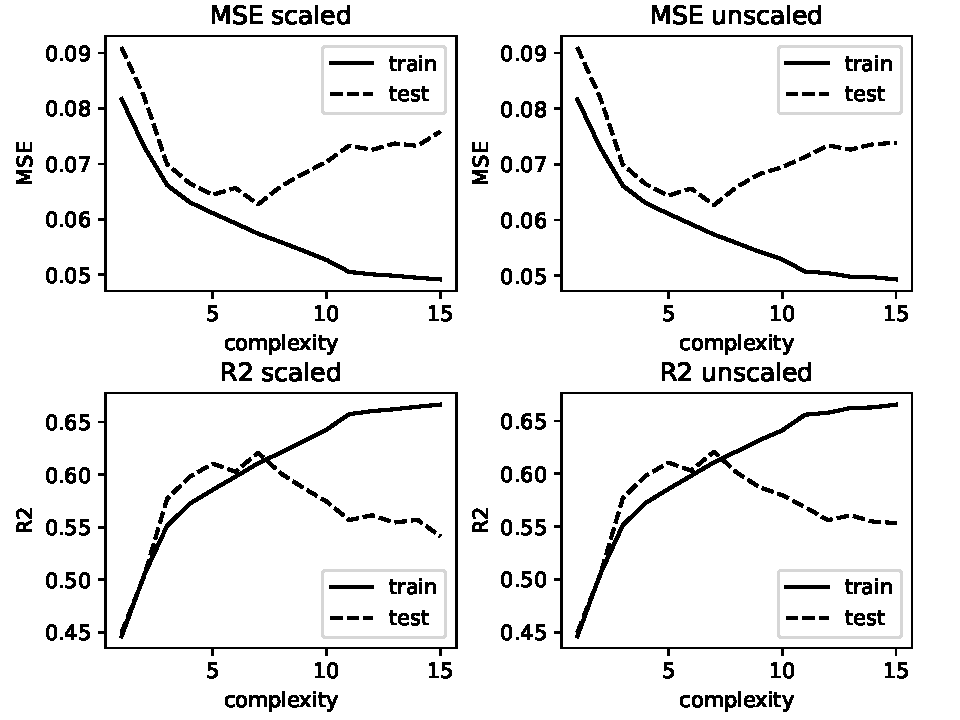
\includegraphics[scale=0.7]{ex1_mse_r2_comp_600_noise_0.25.pdf}
        \caption{MSE and $R^2$ scores for training and testing sets, OLS with polynomial degrees $[1, 15]$. Complexity is here the same as the polynomial degree. $600$ data points were used in the computations. We see that beyond degrees $5$-$7$, the MSE for the training data goes down as we fit more features, while the MSE for the testing data goes up.}
        \label{fig:ex1-1}
    \end{figure}

    Through the analysis of Figure \ref{fig:ex1-1} we find that there seems to be no difference between scaled and unscaled data (by scaling we mean subtraction of the mean value of each column), since the MSEs and $R^2$ scores are identical. This is due to the fact that the values we are trying to fit do not vary a lot, so the effect of scaling is much less noticeable.
    
    The MSE and $R^2$ score of the training and testing sets also behave as expected, Figure 2.11 of Hastie et al., \cite{hastie}. As we increase the complexity of our model, the data involved in the training process is fitted very well, i.e. gives an MSE of nearly $0$ and an $R^2$ score close to $1$. However, when trying to make a prediction to data not included in the training process, as we increase the model complexity, we start to get diminishing returns. This happens since the model will become so tuned for the training data set that adding a point where the model was not trained for will yield a large error (overfitting). We also observe that a $5^{th}$ to $7^{th}$ degree polynomial achieves the best fit, with the test data MSE at its lowest and $R^2$ score at its highest, Figure \ref{fig:ex1-1}.
    
    \begin{figure}[h]
        \centering
        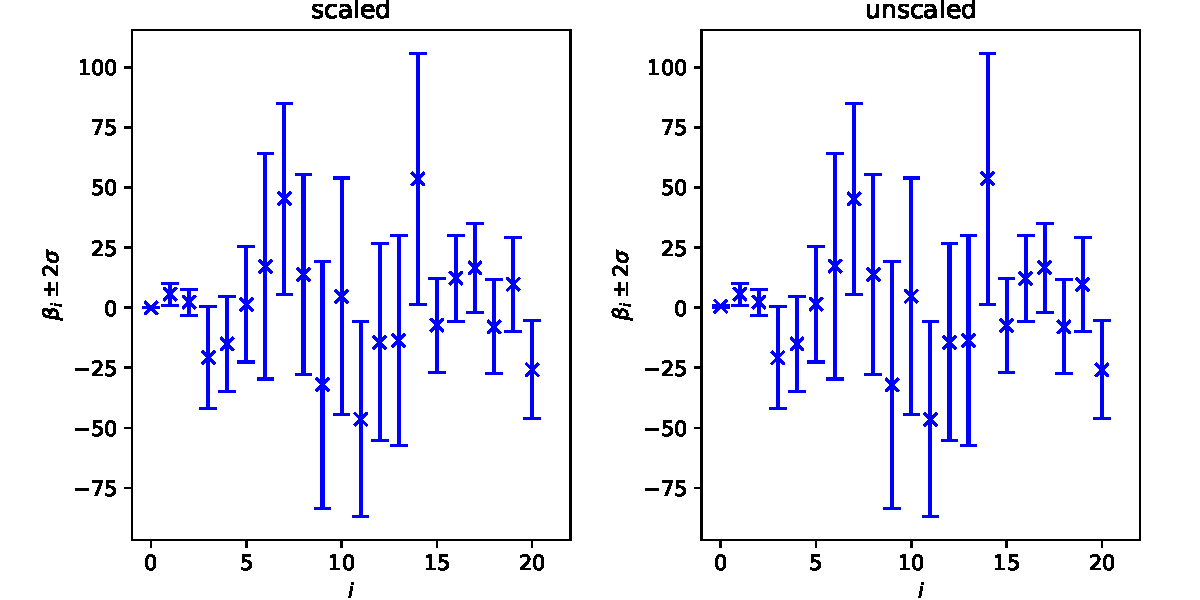
\includegraphics[scale=0.5]{ex1_cnf_intv_betas_n_600_noise_0.25.pdf}
        \caption{Confidence intervals for features $\beta$ in polynomial fit of degree $5$.}
        \label{fig:ex1-2}
    \end{figure}
    
    Lastly, we compute the confidence intervals for the optimal feature parameters $\hat{\beta}$, Equation \eqref{eq:std_betas}, Figure \ref{fig:ex1-2}. The order of magnitude of $\mathbb{E}[\beta_i]$ is the same or less than $\text{std}(\beta_i)$, therefore the estimation of $\bm{\beta}$ is precise. The confidence intervals for the features $\hat{\beta}$ are very similar for both scaled and unscaled predictions, showing again that, in this case, scaling the data does not yield better or worse results.
    
    As referenced before, our data, the Franke function evaluated at $[0,1]\times[0,1]$, lies in a very small interval, hence scaling the data does not have a noticeable effect on reducing the error of our models, as we see in Figure \ref{fig:ex1-1}. As scaling our data (i.e., subtracting the mean value of each column in our case) does not change the fit, we choose to scale it since it removes the intercept column, meaning we do not have to take the intercept into account for further computations with our own implementation and with \texttt{sklearn}'s.

\section*{Exercise 2}

    In this exercise, the aim is to study the bias-variance trade-off, using the OLS method with bootstrap as a resampling technique. In bootstrapping, our goal is to resample the data $M$ times, such that we perform a random sample from the training data, with replacement. We can use this to estimate the probability distribution of our predictors, and assess any measure of accuracy.
    
    In the bias-variance decomposition we want to decompose the mean of the mean squared error (i.e. the cost function in our case) into terms that can be interpreted more clearly. We thus need to look at
    \begin{equation*}
        \mathbb{E}\left[C(X,\bm{\beta})\right] = \mathbb{E}\left[\frac{1}{n}\sum_{i=0}^{n-1}(z_i - \widetilde{z}_i)^2\right] = \frac{1}{n}\mathbb{E}\left[(\bm{z} - \bm{\widetilde{z}})^2\right],
    \end{equation*}
    where \(\bm{z}=\bm{f}+\bm{\epsilon}\) is our data and \(\bm{\widetilde{z}}=X\bm{\beta}\) is our model. We have
    \begin{align*}
        \mathbb{E}\left[(\bm{z} - \bm{\widetilde{z}})^2\right] &= \mathbb{E}\left[(\bm{z} - \mathbb{E}[\bm{\widetilde{z}}] + \mathbb{E}[\bm{\widetilde{z}}] - \bm{\widetilde{z}})^2\right] 
        \\
        &= \mathbb{E}\left[\big(\bm{z} - \mathbb{E}[\bm{\widetilde{z}}]\big)^2\right] - 2\mathbb{E}\Big[(\bm{z} - \mathbb{E}[\bm{\widetilde{z}}])\cdot(\mathbb{E}[\bm{\widetilde{z}}] - \bm{\widetilde{z}})\Big] + \mathbb{E}\left[\big(\bm{\widetilde{z}} - \mathbb{E}[\bm{\widetilde{z}}]\big)^2\right],
    \end{align*}
    where we have defined \(\mathbb{E}[\bm{\widetilde{z}}]=\begin{pmatrix}\mathbb{E}[\widetilde{z}_0] & \mathbb{E}[\widetilde{z}_2] & \ldots & \mathbb{E}[\widetilde{z}_{n-1}]\end{pmatrix}^{T}\). The term \(\mathbb{E}\left[\big(\bm{\widetilde{z}} - \mathbb{E}[\bm{\widetilde{z}}]\big)^2\right]\) can be thought of as the variance of \(\bm{\widetilde{z}}\), therefore we choose to denote it by \(\text{var}(\bm{\widetilde{z}})\). 
    
    Taking a closer look at the second term:
    \begin{align*}
        \mathbb{E}\Big[(\bm{z} - \mathbb{E}[\bm{\widetilde{z}}])\cdot(\mathbb{E}[\bm{\widetilde{z}}] - \bm{\widetilde{z}})\Big] &= \mathbb{E}\left[\sum_{i=0}^{n-1}(z_i - \mathbb{E}[\widetilde{z}_i])(\mathbb{E}[\widetilde{z}_i] - \widetilde{z}_i)\right] = \sum_{i=0}^{n-1}\mathbb{E}\big[(z_i - \mathbb{E}[\widetilde{z}_i])(\mathbb{E}[\widetilde{z}_i] - \widetilde{z}_i)\big]
        \\
        &= \sum_{i=0}^{n-1}\Big(\mathbb{E}\big[(z_i - \mathbb{E}[\widetilde{z}_i])\big]\mathbb{E}\big[(\mathbb{E}[\widetilde{z}_i] - \widetilde{z}_i)\big] + \text{cov}\big(z_i - \mathbb{E}[\widetilde{z}_i],\mathbb{E}[\widetilde{z}_i] - \widetilde{z}_i\big)\Big).
    \end{align*}
    
    As \(\mathbb{E}[\widetilde{z}_i]\) is constant, we see that \(\mathbb{E}\big[(\mathbb{E}[\widetilde{z}_i] - \widetilde{z}_i)\big]=\mathbb{E}[\widetilde{z}_i] - \mathbb{E}[\widetilde{z}_i]=0\). Furthermore, since the covariance is invariant under addition of a number to any of the stochastic variables and that multiplication by a constant goes outside, we find for \(z_i=f_i+\epsilon_i\)
    \begin{align*}
        \text{cov}\big(z_i - \mathbb{E}[\widetilde{z}_i],\mathbb{E}[\widetilde{z}_i] - \widetilde{z}_i\big) = -\text{cov}\big(z_i,\widetilde{z}_i\big) = -\text{cov}\big(f_i + \epsilon_i,\widetilde{z}_i\big) = -\text{cov}\big(\epsilon_i,\widetilde{z}_i\big)
    \end{align*}
    as \(\bm{f}\) is not stochastic. The model \(\bm{\widetilde{z}}\) was found using data independent of \(\bm{\epsilon}\), and we therefore assume that \(\epsilon_i\) is independent of \(\widetilde{z}_i\), i.e., \(\text{cov}\big(\epsilon_i,\widetilde{z}_i\big) = 0\). We are now left with our first expression for the bias-variance decomposition:
    \begin{align*}
        \mathbb{E}\left[(\bm{z} - \bm{\widetilde{z}})^2\right] &= \mathbb{E}\left[\big(\bm{z} - \mathbb{E}[\bm{\widetilde{z}}]\big)^2\right] - 2\overbrace{\mathbb{E}\Big[(\bm{z} - \mathbb{E}[\bm{\widetilde{z}}])\cdot(\mathbb{E}[\bm{\widetilde{z}}] - \bm{\widetilde{z}})\Big]}^{ = 0} + \overbrace{\mathbb{E}\left[\big(\bm{\widetilde{z}} - \mathbb{E}[\bm{\widetilde{z}}]\big)^2\right]}^{ = \text{var}(\bm{\widetilde{z}})}
        \\
        &= \mathbb{E}\big[\bm{z}^2 - 2\bm{z}\mathbb{E}[\bm{\widetilde{z}}] + \mathbb{E}[\bm{\widetilde{z}}]^2\big] + \text{var}(\bm{\widetilde{z}}) = \mathbb{E}\big[\bm{z}^2\big] - 2\mathbb{E}[\bm{z}]\mathbb{E}[\bm{\widetilde{z}}] + \mathbb{E}[\bm{\widetilde{z}}]^2 + \text{var}(\bm{\widetilde{z}}).
    \end{align*}
    
    If now \(\text{var}(\bm{z}) = 0\), then \(\mathbb{E}[\bm{z}^2] = \mathbb{E}[\bm{z}]^2\), and we can write
    \begin{equation*}
        \mathbb{E}\left[(\bm{z} - \bm{\widetilde{z}})^2\right] = \left(\mathbb{E}[\bm{z}] - \mathbb{E}[\bm{\widetilde{z}}]\right)^2 + \text{var}(\bm{\widetilde{z}}) = \text{bias}^2 + \text{var}(\bm{\widetilde{z}}),
    \end{equation*}
    where \(\mathbb{E}[\bm{z}] - \mathbb{E}[\bm{\widetilde{z}}]\) is known as the bias.
    
    Knowing \(\bm{z}=\bm{f} + \bm{\epsilon}\), we obtain
    \begin{align*}
        \mathbb{E}\left[\big(\bm{z} - \mathbb{E}[\bm{\widetilde{z}}]\big)^2\right] &= \mathbb{E}\left[\big((\bm{f} - \mathbb{E}[\bm{\widetilde{z}}]) + \bm{\epsilon}\big)^2\right] = \mathbb{E}\big[(\bm{f} - \mathbb{E}[\bm{\widetilde{z}}])^2 - 2\bm{\epsilon}\cdot(\bm{f} - \mathbb{E}[\bm{\widetilde{z}}]) + \epsilon^2\big]
        \\
        &= \mathbb{E}\big[(\bm{f} - \mathbb{E}[\bm{\widetilde{z}}])^2\big] - 2\overbrace{\mathbb{E}[\bm{\epsilon}]}^{ = \bm{0}}\cdot(\bm{f} - \mathbb{E}[\bm{\widetilde{z}}]) + \mathbb{E}\big[\bm{\epsilon}^2\big] 
        \\
        &= \mathbb{E}\big[(\bm{f} - \mathbb{E}[\bm{\widetilde{z}}])^2\big] + \mathbb{E}[\bm{\epsilon}]\cdot\mathbb{E}[\bm{\epsilon}] + \sum_{i=0}^{n-1}\text{var}(\epsilon_i) = (\bm{f} - \mathbb{E}[\bm{\widetilde{z}}])^2 + n\sigma^2.
    \end{align*}
    
    The bias-variance decomposition for the cost function is therefore
    \begin{equation}
        \mathbb{E}\left[\frac{1}{n}\sum_{i=0}^{n-1}(z_i - \widetilde{z}_i)^2\right] = \frac{1}{n}\overbrace{\sum_{i=0}^{n-1}(f_i - \mathbb{E}[\widetilde{z}_i])^2}^{\text{bias}^2} + \frac{1}{n}\overbrace{\sum_{i=0}^{n-1}\mathbb{E}\left[\big(\widetilde{z}_i - \mathbb{E}[\widetilde{z}_i]\big)^2\right]}^{\text{var}(\bm{\widetilde{z}})} + \sigma^2.
    \end{equation}

    This way, we have shown that we can decompose the error into two main factors, the bias and the variance. The bias is the difference between the mean predictions by our model and the target we are trying to predict. A high bias would indicate a failure for our model to fit the target points, leading to an underfit. The variance is the difference between the mean predictions given by our model and the predictions themselves.
    
    \begin{figure}[h]
        \centering
        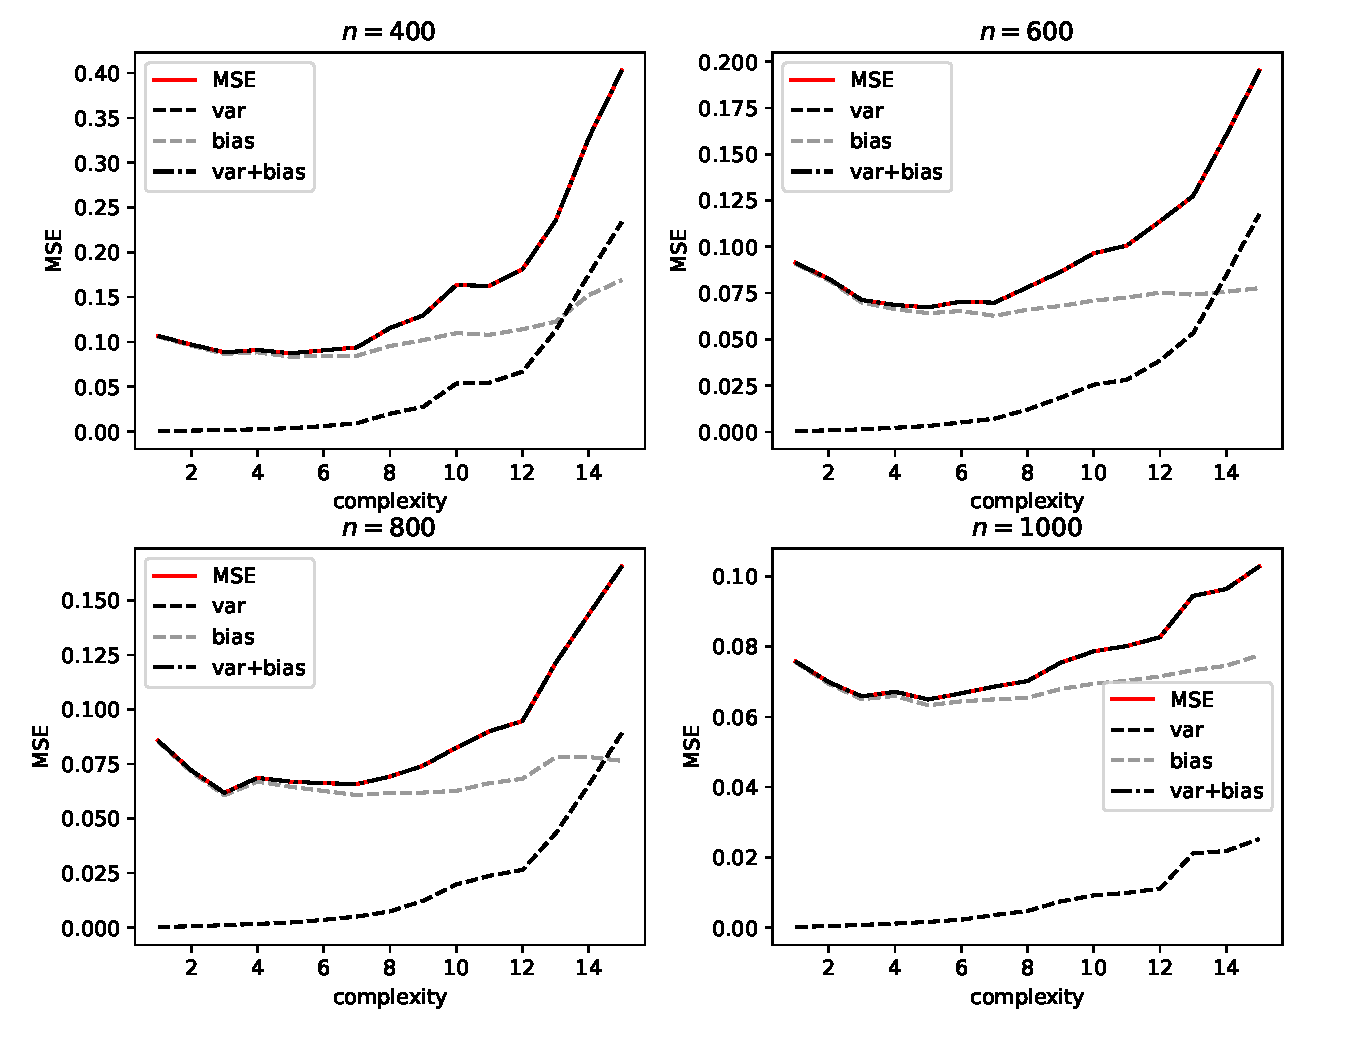
\includegraphics[scale=0.65]{ex2_bias_var_bsc_100_noise_0.25.pdf}
        \caption{Bias-variance trade-off analysis as a function of model complexity, for different number of data points. The number of bootstrap cycles used in the computations is $100$.}
        \label{fig:bv_ols_bs}
    \end{figure}
    
    With low complexity, we expect the model not to fit each point correctly. Thus we would have a high bias and low variance, since the predictions would be far from the real values (high bias) and the model would be easy to generalize for a new data set (low variance). For higher complexities, the predictions will be very close to the accurate target values (low bias), thus the model would become much harder to generalize for a new data set (high variance). In general, we want to achieve a model that has low bias and low variance, since we want to have a good fit for the training and testing data.
    
    In Figure \ref{fig:bv_ols_bs}, we observe the bias and variance of the predicted test data for varying model complexities, using bootstrap as a resampling technique to estimate the bias and variance of the estimators. If we focus on the $n=400$ plot, we observe that for lower complexities we get higher bias and low variance and vice-versa for high complexities. Again, a complexity of $5$ to $7$ would be optimal for this model, as these values result in the lowest MSEs. Shifting our focus to the other plots, we can see that they follow the same trend. As complexity increases, the variance also increases whilst the bias decreases slightly. Thus, we can conclude that an optimal polynomial degree is consistently found to be between $5$ and $7$ for OLS.
    
\section*{Exercise 3}
    
    In exercise $3$ we are tasked to study the bias-variance trade-off for the OLS model using $k$-folds cross-validation as a resampling technique. The $k$-folds cross-validation resampling technique consists of the following steps:
    \begin{enumerate}
        \item If our data is not already randomized, we permute the data.
        \item We divide our data into $k$ equal parts (folds).
        \item Each fold is in turn used as the test set, while the \(k-1\) other folds are used as the training set.
    \end{enumerate}
    
    \begin{figure}[h]
        \centering
        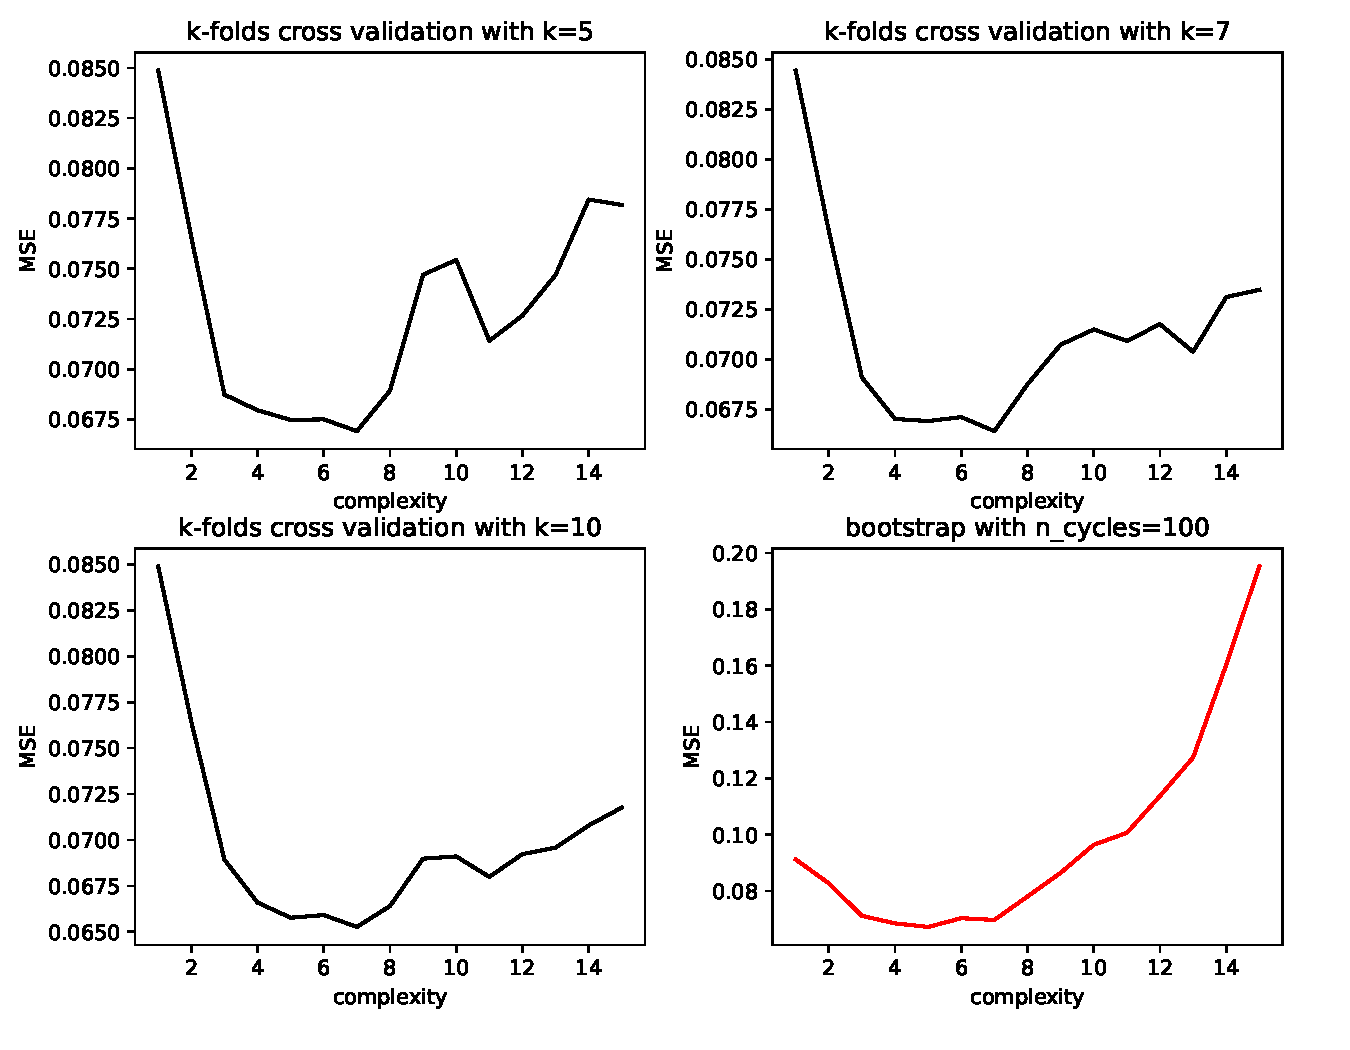
\includegraphics[scale=0.6]{ex3_cv_bs_n_600_noise_0.25.pdf}
        \caption{MSE for various model complexities (polynomial degrees) with $5$, $7$, and $10$ folds and with bootstrap resampling, with $100$ bootstrap cycles. $600$ data points were used in the computations. We see that the results when using cross-validation is fairly consistent, but the error does actually decrease for higher number of folds. Moreover, $k$-folds tends to produce lower MSEs than bootstrap.}
        \label{fig:ex3-1}
    \end{figure}
    
    In figure \ref{fig:ex3-1} we see our results from performing $k$-folds cross-validation for \(k=5,7,10\), compared to the results for bootstrap resampling with $100$ bootstrap cycles. We see here that cross-validation gives quite consistent results, and the MSE is generally smaller then when using bootstrap. The model's estimated accuracy through cross-validation increases slightly when the number of folds is increased. This is expected since we are using more training data and less testing data as we increase the number of folds (and thus decrease their size). Hence the model's error diminishes. A good value for $k$ might be $7$ or $10$, since they seem to give better results than $5$ folds; however, with $10$ folds, we are training with $90\%$ of the data, which could lead to a higher variance. Thus, for the next exercises, when performing $k$-folds cross-validation, we will use $k=7$.
    
    Another noteworthy aspect of this analysis is the computational time it takes to run bootstrap and cross-validation. With bootstrap, depending on the number of bootstrap cycles, the whole process can take a considerable amount of time to finish and reach a solution; with cross-validation, since we only need to loop over the data $k$ times, the process is much quicker.
    
\section*{Exercise 4}

    Having studied the precision of the OLS model to fit the Franke function, we move on to Ridge regression. The Ridge model is more complex and, unlike OLS, has one extra parameter $\lambda$, called a hyperparameter. The cost function in this case is given by
    \begin{equation*}
        C(X, \bm{\beta}) = \frac{1}{n} \left(|| \bm{z} - X\bm{\beta} ||_2^2 + \lambda || \bm{\beta} ||_2^2\right),
    \end{equation*}
    where $||.||_2$ is the $2$-norm, defined as $||\bm{x}||_2^2=\sum x_i^2$. Through the minimization of the cost function, we obtain the analytical expression for Ridge regression
    \begin{equation} \label{eq:beta_ridge}
        \bm{\beta}^{Ridge} = \left(X^T X + \lambda \mathbb{I} \right)^{-1} X^T \bm{z},
    \end{equation}
    where $\bm{\beta}^{Ridge}$ are the optimal $\bm{\beta}$ parameters. Note that, setting $\lambda = 0$, we get the optimal $\bm{\beta}$ expression for Ordinary Least Squares, Equation \eqref{eq:ols_betas}.
    
    Because of this extra parameter, we need to vary not only the complexity, but the value of $\lambda$ as well. Hence, we choose to compute a mesh-grid of polynomial degrees and $\lambda$ values, obtaining a prediction from Ridge regression and calculating the MSE for each one of those points. The range of $\lambda$ values chosen to evaluate the MSE for different complexities here is logarithmically spaced, $\lambda \in [10^{-5}, 10]$. The number of bootstrap cycles and folds chosen are $100$ and $7$, respectively.
    
    \begin{figure}[h]
        \centering
        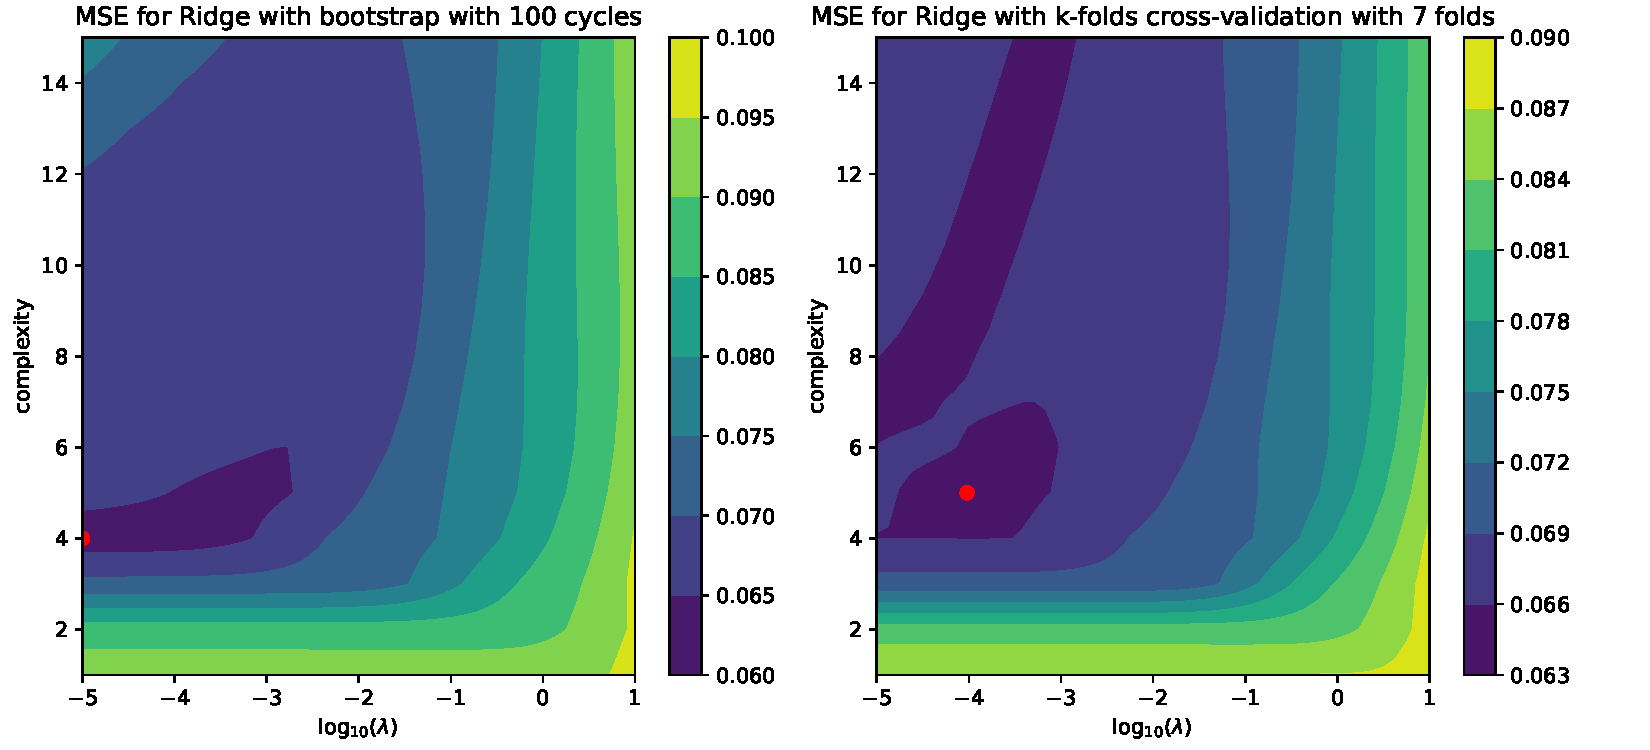
\includegraphics[scale=0.55]{ex4_bs_bcs_100_cv_k_folds_7_n_lmd_50_n_600_noise_0.25.pdf}
        \caption{(left) Contour plot for the MSE for Ridge regression, estimated with bootstrap ($100$ bootstrap cycles), as a function of hyper\-parameter values and model complexities. (right) Contour plot for the MSE for Ridge regression, estimated with $k$-folds cross-validation ($7$ folds), over various $\lambda$ values and model complexities. Regions with darker colours represent the areas where the MSE is smaller. The red point marks the minimum MSE, which gives the optimal values for the hyperparameter and model complexity. The number of data points used here is $600$.}
        \label{fig:ex4}
        % Bootstrap: 
        % mse: 0.061996245301184735; lmd: 1e-05; deg: 4.0 
        % Cross Validation: 
        % mse: 0.065636389692074; lmd: 9.540954763499944e-05; deg: 5.0 
    \end{figure}
    
    Figure \ref{fig:ex4} shows the MSE for predictions given by Ridge regression as a function of the hyperparameter $\lambda$ and the model complexity, given by both bootstrap and cross-validation. For bootstrap, we get $(\lambda_{min}, \text{deg}_{min}) = (1.00 \times 10^{-5}, 4)$ with an MSE of $0.06$, and for cross-validation $(\lambda_{min}, \text{deg}_{min}) = (9.54 \times 10^{-5}, 5)$ with an MSE of $0.07$. 
    
    Since the $\lambda$ values for which we get the lowest MSEs with Ridge regression are very close to zero, these results are comparable with OLS results. With OLS and $k$-folds cross-validation with $k=7$, we get an error approximately of $0.06$ for degrees between $4$ and $7$, Figure \ref{fig:ex3-1}. These results are very close to what we get with Ridge regression, without having to account for an extra parameter. Hence we can say that OLS is able to create a better fit for the Franke function.
    
    Another noteworthy aspect is that the estimators with Ridge regression take more time to compute with lower values of $\lambda$, but OLS takes even less time to compute. This shows again that OLS is a better option than Ridge to fit the Franke function on this interval.
    
\section*{Exercise 5}
    
    In this exercise, we study the bias-variance trade-off with Lasso regression. Like Ridge, Lasso regression also depends on a hyperparameter $\lambda$ that can vary. The cost function for Lasso regression is given by
    \begin{equation*}
        C(X, \bm{\beta}) = \frac{1}{n} \left(|| \bm{z} - X\bm{\beta} ||_2^2 + \lambda || \bm{\beta} ||_1\right),
    \end{equation*}
    where $||\cdot||_2$ is again the $2$-norm, and $||\cdot||_1$ is the 1-norm, defined as $||\bm{x}||_1=\sum_{i=0}^n |x_i|$. This is very similar to the cost function for Ridge regression; the only difference is that with Lasso we multiply $\lambda$ by the $1$-norm of the features vector $\beta$. Through the minimization of the cost function we can obtain the optimal $\bm{\beta}$ values. In this case the analytical solution is more complicated and difficult to compute, we can write
    \begin{equation} \label{eq:beta_lasso}
        \bm{\beta}^{Lasso} = \text{argmin}\left( || \bm{z} - X\bm{\beta} ||_2^2 + \lambda || \bm{\beta} ||_1 \right),
    \end{equation}
    where $\bm{\beta}^{Lasso}$ are the optimal $\bm{\beta}$ parameters. Again, if we set $\lambda = 0$, then we will get the optimal $\bm{\beta}$ expression for Ordinary Least Squares, Equation \eqref{eq:ols_betas}.
    
    Since the analytical expression for Lasso regression for the optimal $\bm{\beta}$ is more difficult to compute than Ridge, Equation \eqref{eq:beta_ridge}, and than OLS, Equation \eqref{eq:ols_betas}, numerical methods are used to estimate the minimum of Equation \eqref{eq:beta_lasso}. Here we use \texttt{sklearn}'s implementation for Lasso regression. This implementation uses a gradient descent method to evaluate the minimum of Equation \eqref{eq:beta_lasso}. We have set a tolerance of $0.1$ and a max iteration count of $10^7$, to ensure that the method converges to a stable solution in a reasonable amount of time. Like Ridge regression, Lasso converges faster for larger values of $\lambda$.
    
    \begin{figure}[h]
        \centering
        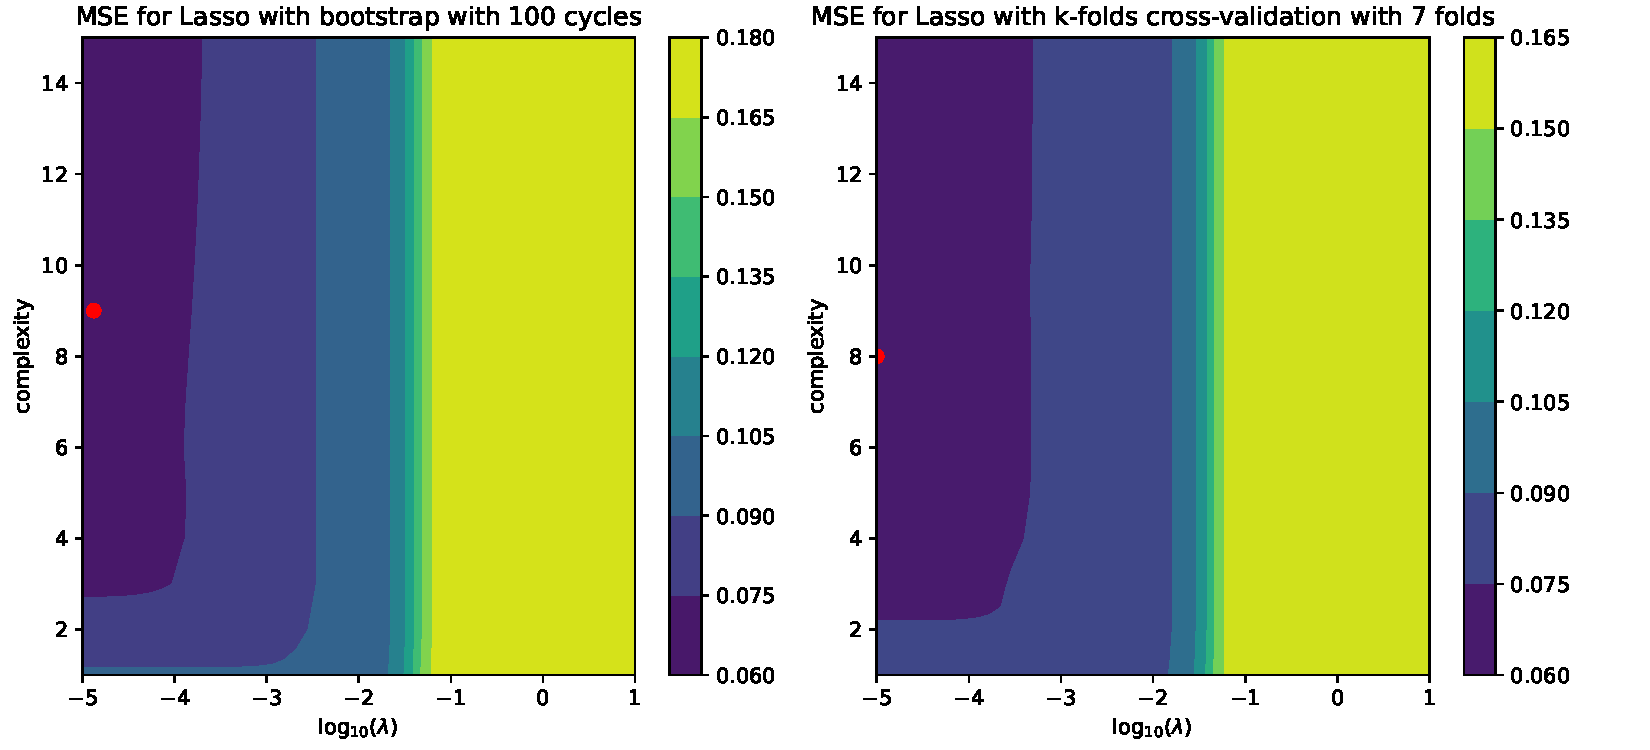
\includegraphics[scale=0.55]{ex5_bs_bcs_100_cv_k_folds_7_n_lmd_50_n_600_noise_0.25.pdf}
        \caption{(left) Contour plot for the MSE for Lasso regression, estimated with bootstrap ($100$ bootstrap cycles), as a function of hyper\-parameter values and model complexities. (right) Contour plot for the MSE for Lasso regression, estimated with $k$-folds cross-validation ($7$ folds), over various $\lambda$ values and model complexities. Regions with darker colours represent the regions where the MSE is smaller. The red point marks the minimum MSE, which gives the optimal values for the hyperparameter and model complexity. The number of data points used is $600$.}
        \label{fig:ex5}
        % Bootstrap: 
        % mse: 0.06745260501884916; lmd: 1.3257113655901082e-05; deg: 9.0 
        % Cross Validation: 
        % mse: 0.06608244728789159; lmd: 1e-05; deg: 8.0 
    \end{figure}
    
    For this exercise, we choose the same interval for the hyperparameter to evaluate the error of Lasso regression, logarithmically spaced $\lambda \in [10^{-5}, 10]$. Figure \ref{fig:ex5} shows two contour plots of the MSE for different $\lambda$ and complexity values, estimated with the bootstrap resampling technique with $100$ bootstrap cycles, and with $k$-folds cross-validation, with $k=7$.
    
    The region of minimal MSEs is found to be very similar to results obtained via Ridge regression. From bootstrap we obtain the minimum MSE of $0.07$ at $(\lambda_{min},\text{deg}_{min}) = (1.33 \times 10^{-5}, 9)$, and from $k$-folds cross-validation we obtain the minimum MSE of $0.07$ at $(\lambda_{min},\text{deg}_{min}) = (1.00 \times 10^{-5}, 8)$. Again, since the $\lambda$ values for which the MSE is minimum are very small ($\lambda_{min} \approx 0$) we compare the results with the results from OLS, Figure \ref{fig:ex3-1}. As the minimum MSE values and corresponding model complexity that we get with OLS are very similar to what we get with Lasso and Ridge, and the computation times with OLS are much lower we can say with certainty that OLS is the better model to fit the Franke function.

    \hypertarget{ridgevlasso}{It is worth noting that the MSE from Lasso regression for $\lambda > 10^{-1}$ is significantly larger than what we get for Ridge, as seen in Figure \ref{fig:ex4}. This may be due to the fact that we have an exact solution for the minimization of Ridge's cost function, Equation \eqref{eq:beta_ridge}, while with Lasso we approximate its minimum value. Since our tolerance for the gradient descent method is very large, $10^{-1}$ (usually it is set to $10^{-7}$), we might get worse results when the additional term in Equation \eqref{eq:beta_lasso} ($\lambda || \bm{\beta} ||_1$) starts to get larger, i.e. when $\lambda$ increases}.

\section*{Exercise 6}
    
    Having explored and analysed the ability of different linear models to fit the Franke function, we proceed to study real data from Norway's vast landscape and repeat the same analysis. For this we use terrain data extracted from \url{https://earthexplorer.usgs.gov/}.
    
    %To load the data into our python script we used the code provided in the Assignment Sheet.
    % ^ we didn't, i wrote the import function :P the sample provided was no good
    % yes but it was based on code provided by morten, the imgread, then it was all what you wrote v that is down there (downsample and scissoring)
    % i mean imageio is pretty much the standard way to load an image in python afaik
    
    The original data spans over 6.4 million data points. If we wanted to fit a linear model to the whole data, we would have to invert a matrix with dimensions $6.4M \times p$. This is computationally expensive since the commonly used matrix inversion algorithms (SVD, LU decomposition, etc.) have a time complexity of $\mathcal{O}(n^3)$ (here $n$ is the dimension of the matrix we want to invert, $A \in \mathbb{R}^{n \times n}$), at best. Because of this, we add a \texttt{downsample} factor when reading the data. This factor acts as a step when reading the data, by only reading data spaced \texttt{downsample} indices apart in the terrain data matrix. This way we are able to represent the entire set, but with an inferior resolution (nearest-neighbour filtering). In Figure \ref{fig:ex6-downsample_only} we can see the whole terrain downsampled by a factor of $20$; $5\%$ of the original points are present, leaving us with about $8000$ data points.
    
    \begin{figure}[h]
        \centering
        \begin{subfigure}{.49\textwidth}
            \centering
            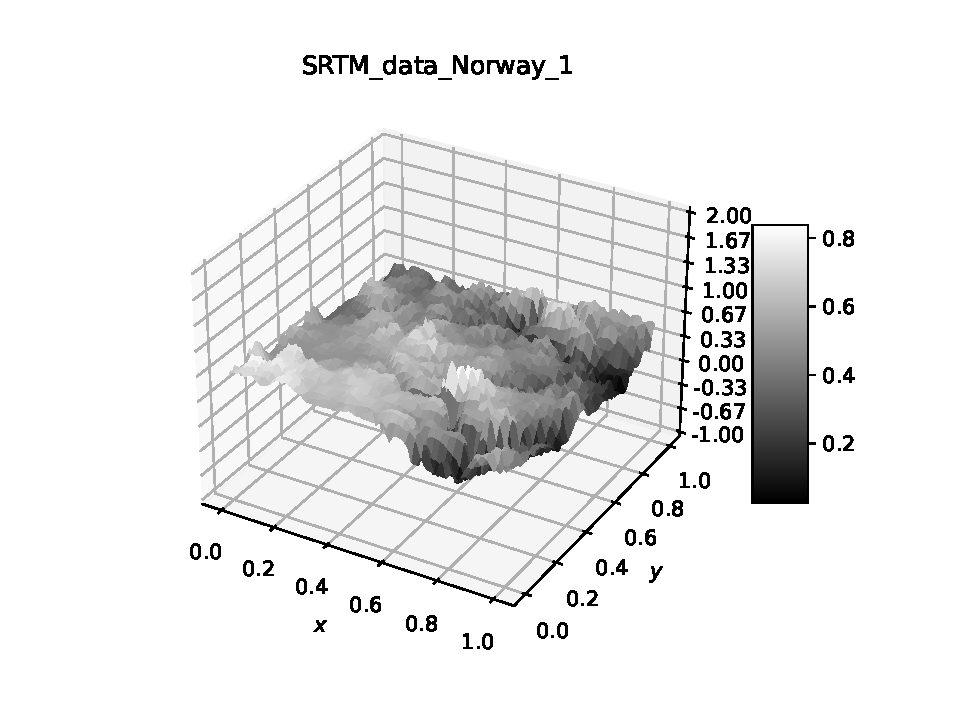
\includegraphics[scale=0.45]{old_ex6/ex6_original_data.pdf}
            \caption{Original terrain data with a \texttt{downsample} factor of $20$. About $8000$ data points.} 
            \label{fig:ex6-og_ds}
        \end{subfigure}
        \begin{subfigure}{.49\textwidth}
            \centering
            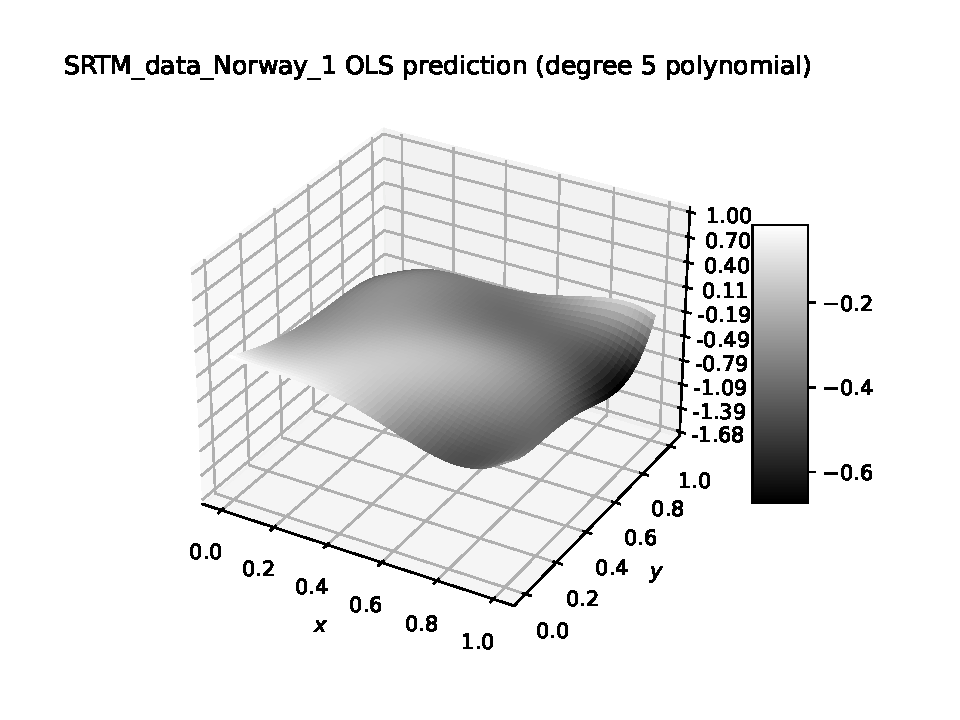
\includegraphics[scale=0.45]{old_ex6/ex6_pred_OLS.pdf} 
            \caption{$5^{th}$ degree polynomial fit to the terrain data with OLS.}
            \label{fig:ex6-pred_ds}
        \end{subfigure}
        \caption{Side-by-side comparison of original full data and prediction for a \texttt{downsample} factor of $20$.}
        \label{fig:ex6-downsample_only}
    \end{figure}
    
    By comparing Figure \ref{fig:ex6-pred_ds} to Figure \ref{fig:ex6-og_ds}, we can see that the prediction by our model does not reproduce the original data with much accuracy. This is due to the terrain being very vast and the model having to account for every single hill, cliff, and valley. We could compute a higher degree polynomial to counter this issue.
    
    Instead, we select a smaller portion of the terrain to study in more detail, Figure \ref{fig:ex6-og}. To do this, we introduce another parameter \texttt{scissor} to crop a portion of the terrain starting at the origin of our coordinate system (northwestern point).
    
    \begin{figure}[h]
        \centering
        \begin{subfigure}{.49\textwidth}
            \centering
            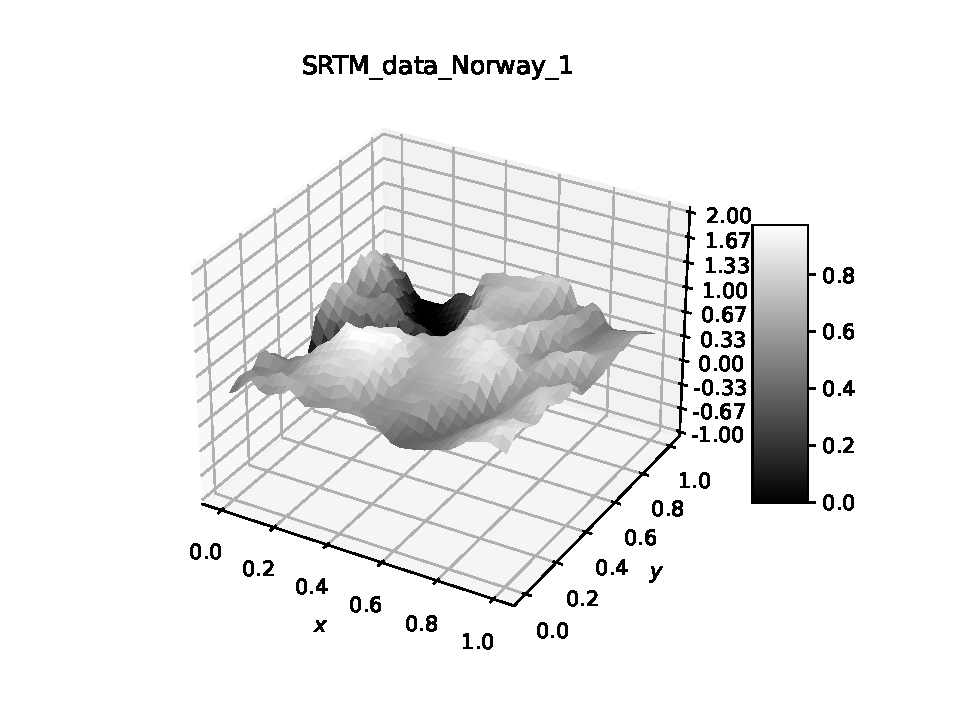
\includegraphics[scale=0.45]{ex6_original_data.pdf}
            \caption{Cropped terrain data with a \texttt{downsample} factor of $14$. $676$ data points.} 
            \label{fig:ex6-og}
        \end{subfigure}
        \begin{subfigure}{.49\textwidth}
            \centering
            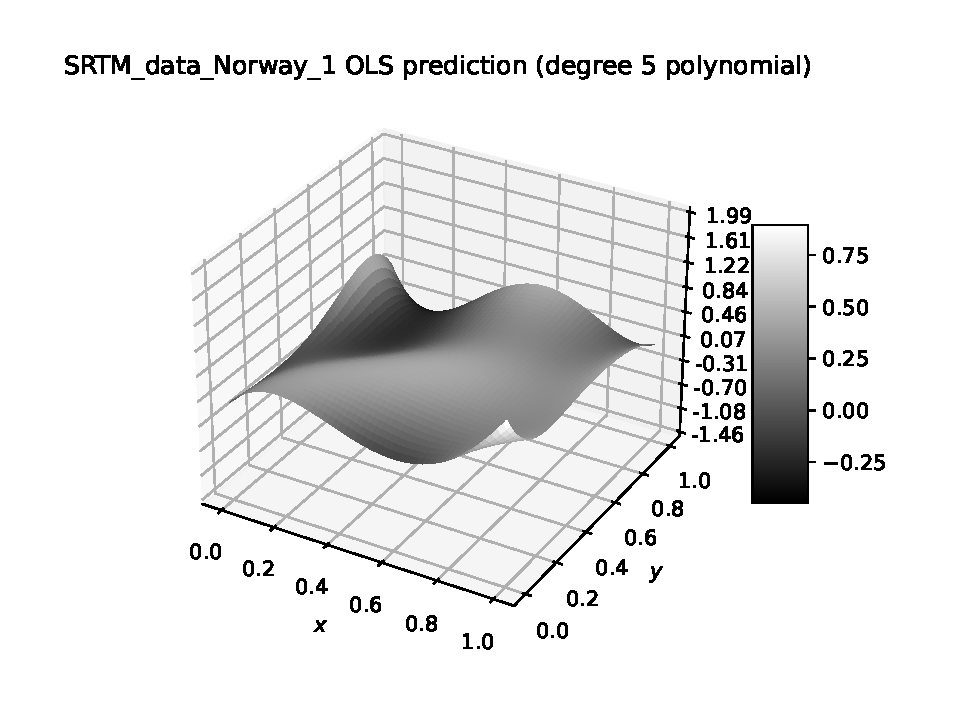
\includegraphics[scale=0.45]{ex6_pred_OLS.pdf} 
            \caption{$5^{th}$ degree polynomial fit to the cropped terrain data with OLS.}
            \label{fig:ex6}
        \end{subfigure}
        \caption{Side-by-side comparison of cropped data and prediction for a \texttt{downsample} factor of $14$ and \texttt{scissoring} factor of $0.20$.}
        \label{fig:ex6}
    \end{figure}
    
    We implement our function to load terrain data, \texttt{load\_terrain} in \texttt{terrain.py}, to support cropping and downsampling of the original data points into a workable subset, in order to keep computation time manageable. All calculations shown below can be reproduced on the full set by setting \texttt{scissor = 1.0} and \texttt{downsample = 1}; provided enough computing power, this will yield the best possible results. We use \texttt{scissor = 0.2} (i.e. the top-left $20\%$ of the image) and \texttt{downsample = 14}. When we want to compare the error for different amount of data points we set \texttt{downsample} between \texttt{10} and \texttt{7}.
    
    First, we use OLS to fit the terrain data (1089 data points) for polynomial degrees $[1, 40]$, for both scaled and unscaled inputs, and compare the MSE and $R^2$ score (Figure \ref{fig:ex6-mse}) for the training and testing sets. We find equivalent results for scaled and unscaled data in lower polynomial degrees, but observe higher test MSEs for higher complexities for predictions on unscaled data; although the gap is still relatively small for polynomials of order $< 40$. In the rest of our analysis of the terrain data, we use exclusively scaled data to make predictions.
    
    \begin{figure}[h] % ex1
        \centering
        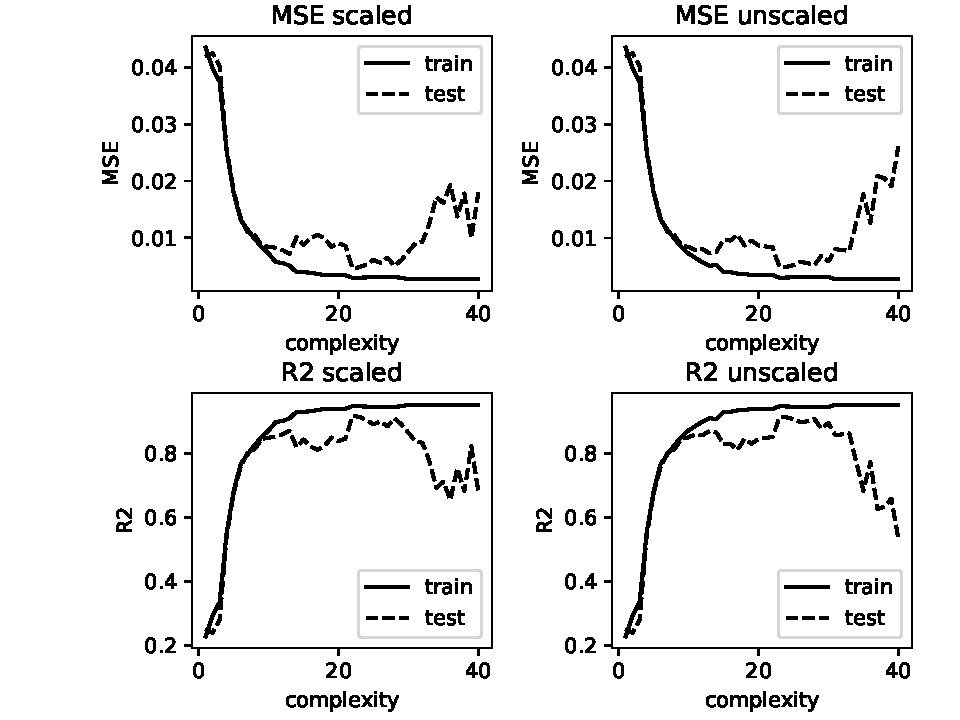
\includegraphics[scale=0.7]{ex6_mse_r2_comp.pdf}
        \caption{MSE and $R^2$ scores for training and testing sets, OLS with polynomial degrees $[1, 40]$}
        \label{fig:ex6-mse}
    \end{figure}
    
    We then study the bias-variance trade-off with bootstrap, with 100 resamples and varying amounts of data points; Figure \ref{fig:ex6-bv}. Again, we find a tendency for lower variance and higher bias for low polynomial degrees and the opposite for higher complexities, although this isn't as clear-cut here as it is for the Franke function fit, likely due to the high potential for discontinuities in the data set. We find optimal polynomial degrees to predict the terrain data to be fairly consistently in the $[10, 25]$ range here.
    
    \begin{figure}[h] % ex2
        \centering
        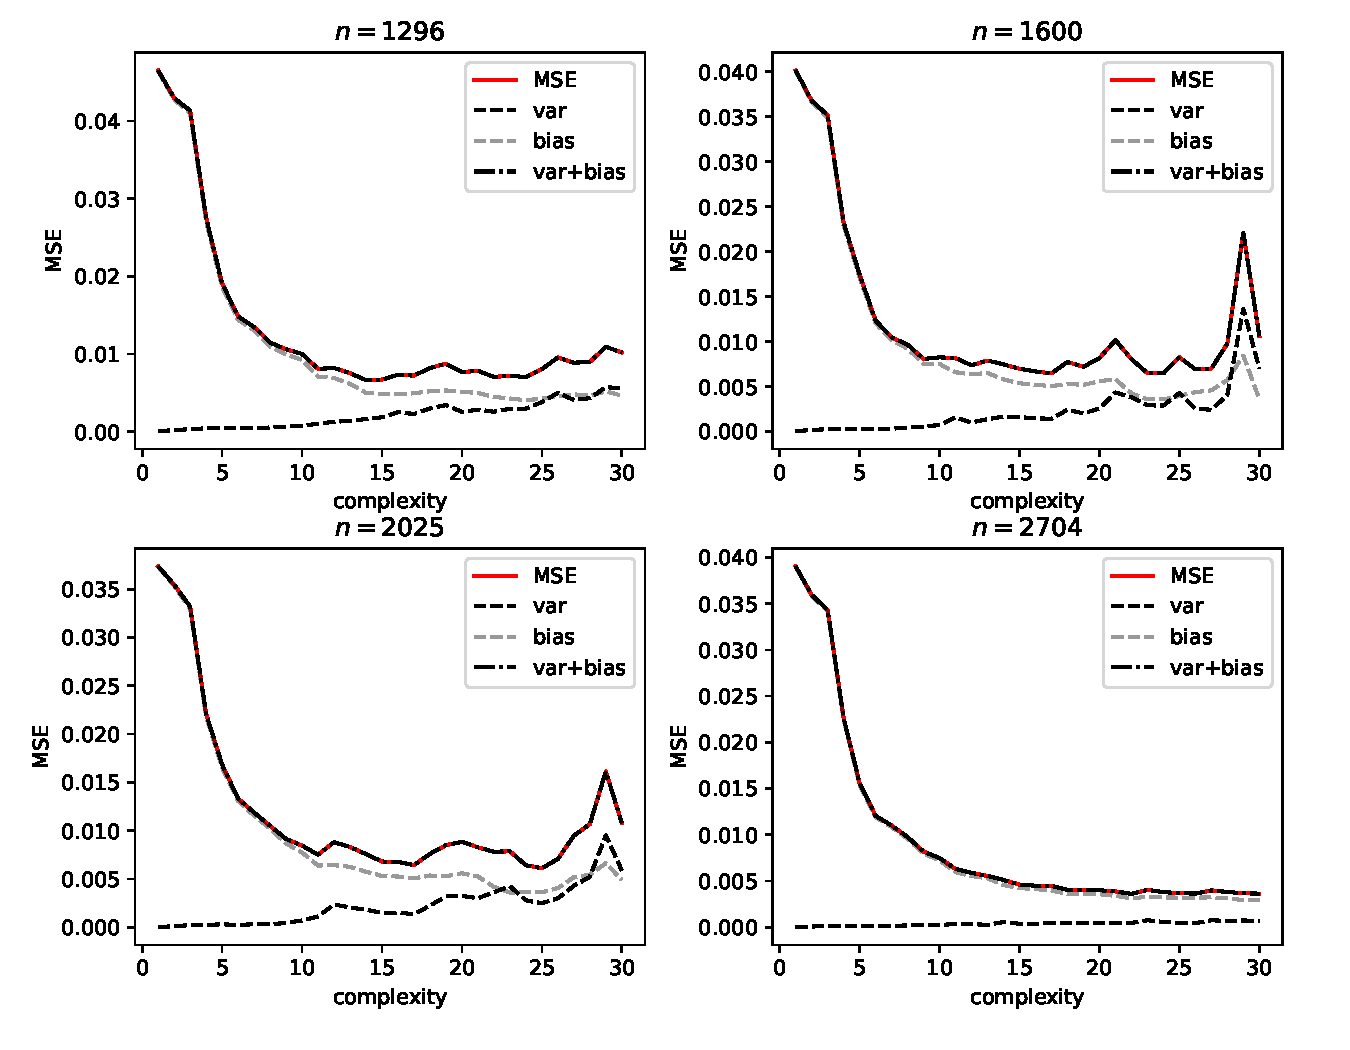
\includegraphics[scale=0.6]{ex6_bias_var_bsc_100_noise_1.0.pdf}
        \caption{Bias-variance trade-off analysis as a function of the polynomial degree, for different number of data points; 100 bootstrap cycles}
        \label{fig:ex6-bv}
    \end{figure}
    
    In Figure \ref{fig:ex6-bvols}, we provide a comparison of $k$-folds cross-validation (7 folds) and bootstrap on the terrain data; we find again a higher degree of accuracy through $k$-folds, although the results are equivalent for both methods. Here, fewer data points are used than in Figure \ref{fig:ex6-bv}, and we find optimal polynomial degrees to be in the $[10, 15]$ range, confirming that predictions suffer from less overfitting for lower-order polynomials.
    
    \begin{figure}[h] % ex3
        \centering
        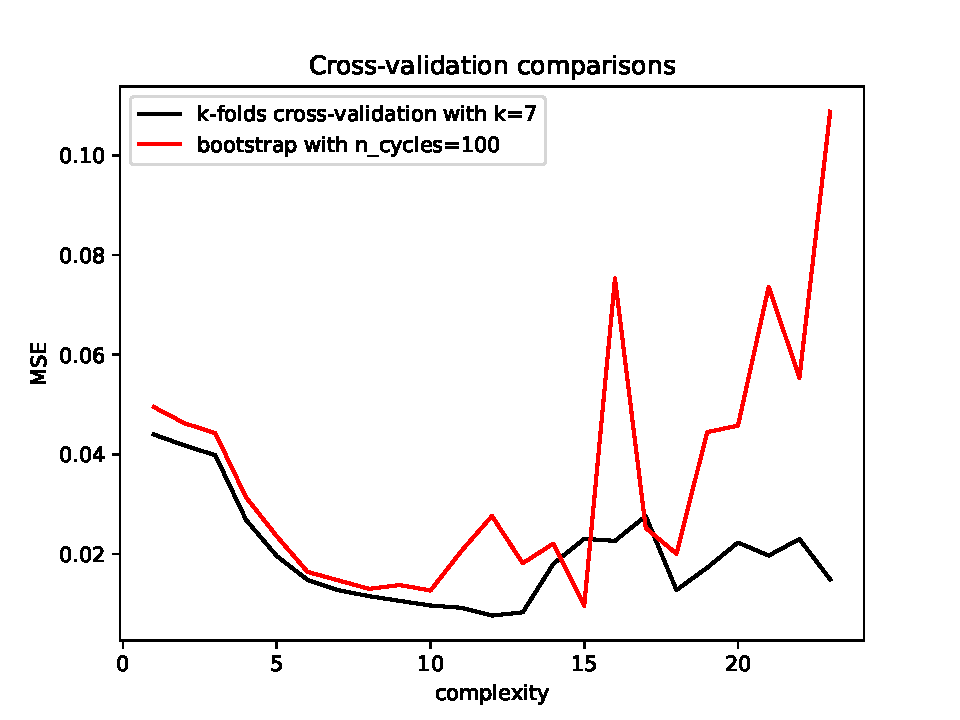
\includegraphics[scale=0.55]{ex6_bv_bootstrap_cv_comp.pdf}
        \caption{MSE for various polynomial degrees with 7-fold $k$-folds cross-validation, and 100-cycle bootstrap; 676 data points used here}
        \label{fig:ex6-bvols}
    \end{figure}
    
    We compute the MSE for the same model, with Ridge and Lasso regression as a function of hyper-parameter $\lambda \in [10^{-5}, 10]$ and polynomial degree (in $[1, 25]$); Figures \ref{fig:ex6-bvridge} and \ref{fig:ex6-bvlasso}. For both models, $k$-folds and bootstrap produce equivalent results. These are also close to Figures \ref{fig:ex4} and \ref{fig:ex5}, although the minimums are found here for higher degrees and lower $\lambda$ values. The minimum MSE is found for Ridge at $\lambda = 10^{-5}$, degree $= 25$ ($MSE_{bootstrap} \approx 9.58 \times 10^{-3}, MSE_{k-folds} \approx 9.16 \times 10^{-3}$), and for Lasso at $\lambda = 10^{-5}$, degree $= 21$ ($MSE_{bootstrap} \approx 15.91 \times 10^{-3}, MSE_{k-folds} \approx 15.79 \times 10^{-3}$).
    
    Again, we observe much higher MSEs for higher $\lambda$ values for Lasso as opposed to Ridge; \hyperlink{ridgevlasso}{recall explanation in section 5}.
    
    \begin{figure}[h] % ex4
        \centering
        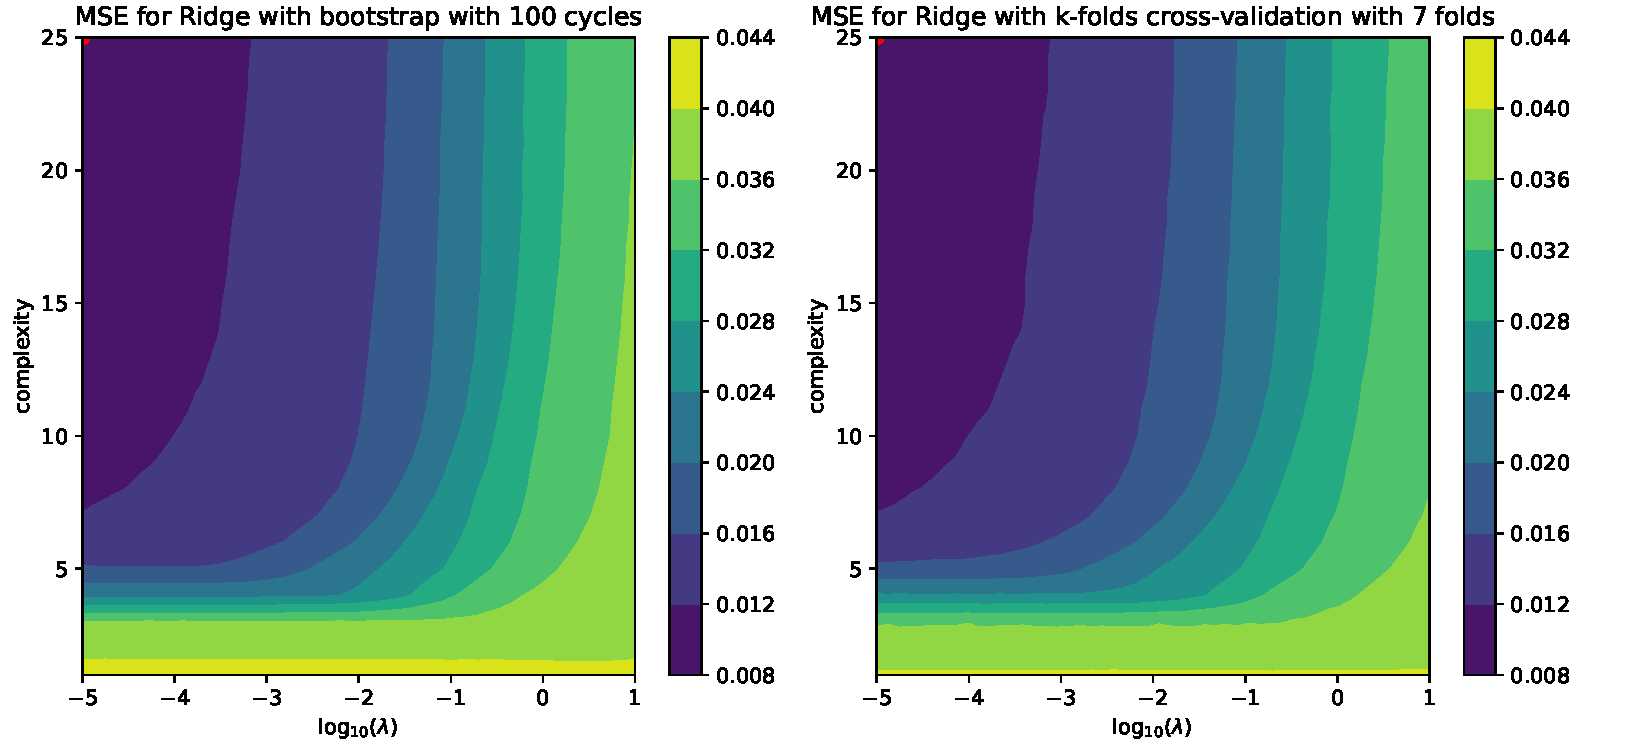
\includegraphics[scale=0.5]{ex6_bs_bcs_100_cv_k_folds_7_n_lmd_50_ridge.pdf}
        \caption{Contour plot for the MSE for Ridge regression, estimated with bootstrap (100 resamples; left) and $k$-folds (7 folds; right) as a function of hyper-parameter values and model complexity; 1089 data points}
        \label{fig:ex6-bvridge}
    \end{figure}
    % Bootstrap: 
    % mse: 0.009579290480381806; lmd: 1e-05; deg: 25.0 
    % Cross Validation: 
    % mse: 0.00915636971469628; lmd: 1e-05; deg: 25.0 

    \begin{figure}[h] % ex5
        \centering
        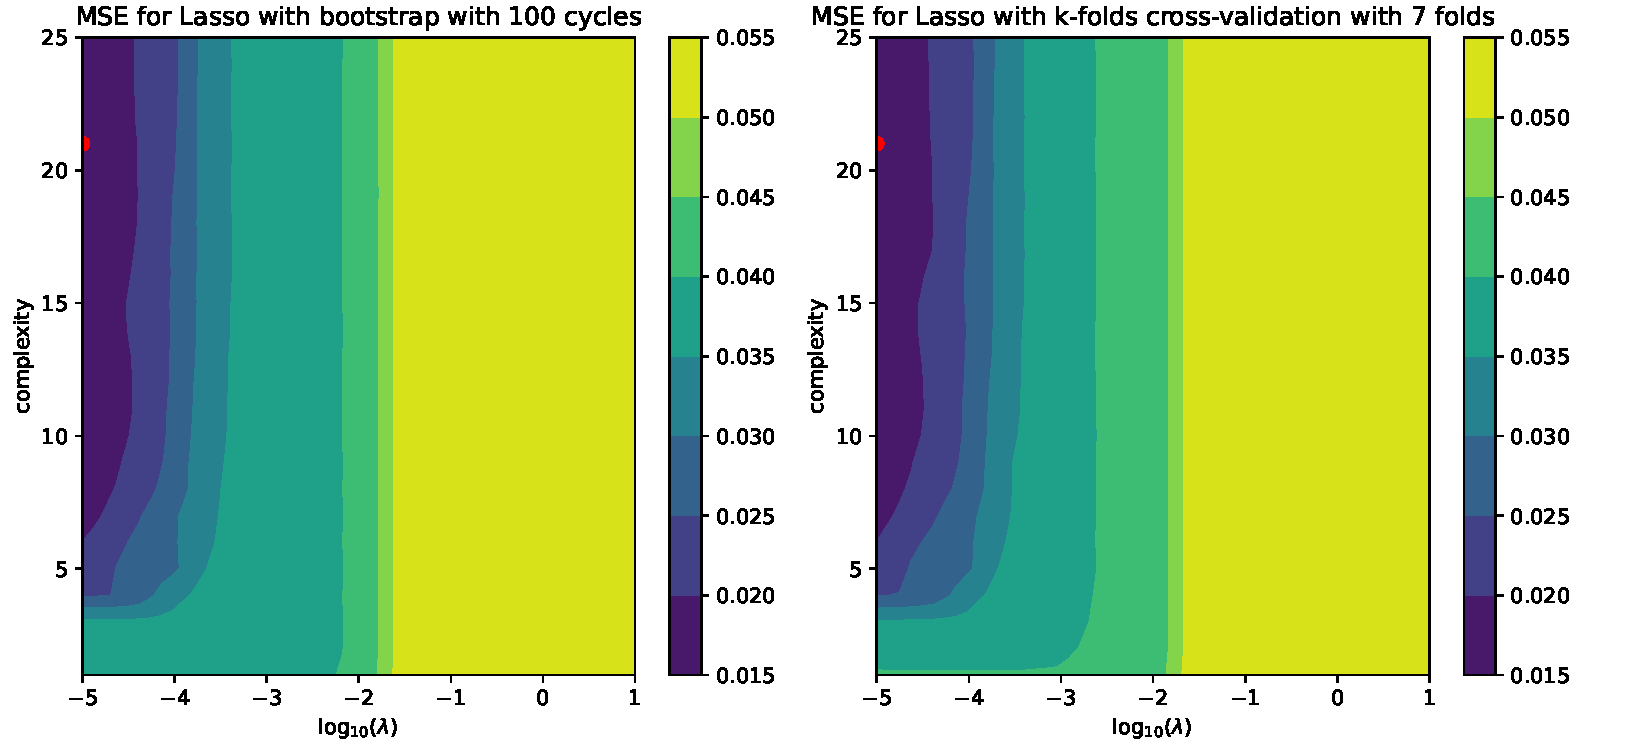
\includegraphics[scale=0.5]{ex6_bs_bcs_100_cv_k_folds_7_n_lmd_50_lasso.pdf}
        \caption{Contour plot for the MSE for Lasso regression, estimated with bootstrap (100 resamples; left) and $k$-folds (7 folds; right) as a function of hyper-parameter values and model complexity; 1089 data points}
        \label{fig:ex6-bvlasso}
    \end{figure}
    % Bootstrap: 
    % mse: 0.015914055585726932; lmd: 1e-05; deg: 21.0 
    % Cross Validation: 
    % mse: 0.015794425542924186; lmd: 1e-05; deg: 21.0 
    
    We observe once again the same pattern as for the Franke function, where OLS produces predictions of equivalent or better precision than Ridge and Lasso regression. As OLS takes considerably less time to compute, we can conclude that the Ordinary Least Squares regression model is the best model to fit the terrain data from this particular section of the Norwegian landscape.
    
    In order to obtain even better predictions of a large section of terrain data, it may be possible to predict polynomial fit for every surface patch for subsections of the landscape and extrapolate with each other to produce the full landscape.

\clearpage

\bibliography{refs}
\bibliographystyle{plain}

\end{document}
